\documentclass[
	english,
	fontsize=10pt,
	parskip=half,
	titlepage=true,
	DIV=12
]{scrartcl}

\usepackage[utf8]{inputenc}
\usepackage{babel}
\usepackage[T1]	{fontenc}
\usepackage{lmodern}
\usepackage{microtype}
\usepackage{color}
\usepackage{csquotes}
\usepackage{tabto}

\usepackage{hyperref}

\usepackage{graphicx}
\usepackage{wrapfig}
\usepackage[bf]{caption}
	\captionsetup{format=plain}

\newcommand*{\tabcrlf}{\\ \hline}

\usepackage{amsmath}

\usepackage{minted}
	\usemintedstyle{friendly}

\newcommand*{\inPy}[1]{\mintinline{python3}{#1}}
\newcommand*{\ie}{i.\;e. }
\newcommand*{\eg}{e.\;g. }

\newcommand{\thus}{\ensuremath{\rightarrow}}

\begin{document}

\part*{Python Problems 06, Winter 2021/22}
\section{Erroneous Code (1\;P)}
Explain, why the below code does \emph{not} work, \ie why in the output, \texttt{x} and \texttt{y} are not swapped.
\begin{minted}[linenos]{python}
def swap(x, y): 
    temp = x
    x = y
    y = temp
  
# Driver code 
x = 2
y = 3
swap(x, y) 
print(x) 
print(y) 
\end{minted}

\section{$\pi$ from the Monte Carlo Method (1\;P)}
\begin{wrapfigure}{r}{.25\linewidth}
\vspace{-20pt}
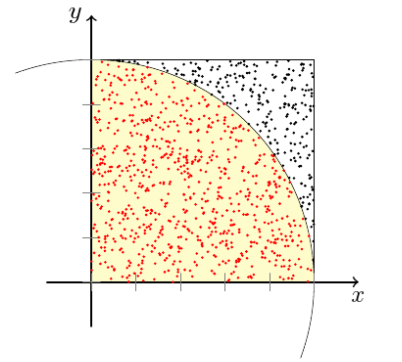
\includegraphics[width=\linewidth]{MCarlo}
\caption{\url{https://commons.wikimedia.org/wiki/File:Pi_statistisch.png}}
\label{fig:MCPI}
\vspace{-40pt}
\end{wrapfigure}
%
Write a function that returns an approximation to the value of $\pi$. To do so, follow these instructions:
\begin{itemize}
\item Generate $N$ pairs of positive random numbers $x, y$ between 0 and 1.
\item For each pair of numbers, compute $x^2 + y^2$
\item For each pair $(x, y)$ where this expression is less than or equal to one, increase a counter.
\item For big $N$, the expression $\frac{\text{counter}}{N}$ approaches $\frac{\pi}{4}$
\end{itemize}

Write your function such that you can pass $N$ as an argument. This parameter controlls the accuracy of your approximation of $\pi$.

\emph{Note}: You'll need \emph{very} big values of $N$ to get half-decent results. If your algorithm outputs something like $3.13$, you've probably done everything correctly.

\emph{Background Information}:\\
Using Pythagoras' theorem, we find that the distance between the origin $(0, 0)$ and some point $(x, y)$ can be computed from
\[ R^2 = x^2 + y^2 \]
If we now fix some value for $R$, we can compute for any point $(x, y)$ whether it is within or outside of a circle of radius $R$. For simplicity, we choose $R = 1$. Since $1^2 = 1$, we find that the algorithm described above counts how many points are within a circle of radius 1.

We are randomly picking points $(x, y)$ from the interval $[0, 1] \times [0, 1]$, \ie a square of unit length, coinciding with the first quadrant of the unit circle centered in origin (cf. figure \ref{fig:MCPI}). Counting the number of dots within the circle amounts to measuring the \emph{area of a quadrant of the circle} in units of the \emph{area of the square}.

As you know, for the area of the circle, it holds:
\[ A = R^2 \cdot \pi \]

Plugging in $R^2 = 1$ and acounting for the factor 4 (we're only covering a quadrant of the circle) gives the above algorithm.

\emph{Background Information}:\\
Monte Carlo Methods are a collection of techniques often used where accuracy has to be sacrificed for computation time. Albeit not terribly precise, they often are the only means of evaluating some integrals. We'll do a mini excursion on them at the end of our course.

\section{Integral (I) (1 P)}
\begin{wrapfigure}{r}{.3\linewidth}
	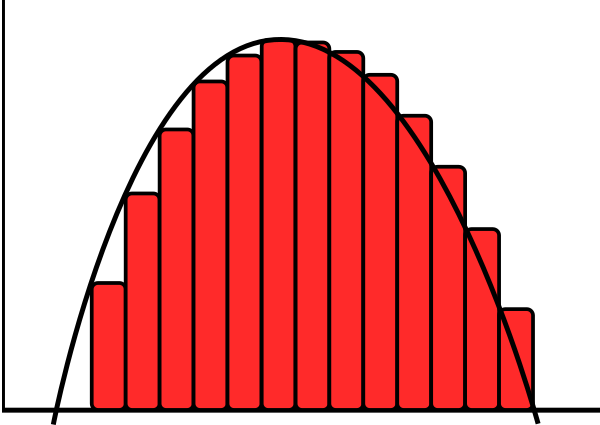
\includegraphics[width=\linewidth]{./integral}
	\caption{Approximation of an integral by area of rectangles.\newline
		Figure by Jonas Süskind}
	\vspace{-50pt}
\end{wrapfigure}
Write a function \texttt{integrate} that approximates the area underneath a graph of a function $f$, \ie compute the value
\[ \int_a^b f(x) \;\text{d}x \]

The integrand $f$ (\ie the function that gives the graph) should be a parameter to your function \texttt{integrate}. Make it such that your function has the signature:
\mint{python}{def integrate(func, start, stop, N) :}

Use the rectangle approximation:
\begin{itemize}
\item Disect the integration interval into $N$ blocks of equal width
\item For each block, evaluate the function $f$ at the left hand side of your block. This gives the height of the rectangles
\item Find the areas of all $N$ rectangles and sum them up -- this gives you an approximation of the integral
\end{itemize}

You can test your code with the following call:
\mint{python}{print( integrate(math.exp, 0, 1, 10000) )}
The output should, approximately, be \texttt{1.718}.


\section{Random/Drunk Walk (2 + 3\;P)}
Imagine a drunkard, stumbling down a road. With each step forward, the drunkard will stagger randomly to the left or right.

Write a program that simulates how far the drunkard has veered off to the left or right after $N$ steps forward. For the basic version of this problem, we'll assume that the drunkard is stumbling along a road of \emph{infinite width}, \ie going to either direction is always possible. Assume now, the drunkard is a bit lopsided: the probability of going left/right is not necessarily 50/50, but \eg 40/60 or any other distribution.

Make it such that your algorithm has the form of a function. The number of steps $N$ and the bias (probability of taking a step to the left) should be a parameters for the function. The return value should be the position of the drunkard after going forward $N$ steps. This position can be represented by an \inPy{int}, stating how many steps right of the starting point the drunkard ended up.

\emph{Optional (+1 P)}:\\
Drop the assumption that the road has infinite width; instead, include a parameter $W$ in your model. Your drunkard starts in the middle of the road. If they have veered off $^{W}/_{2}$ steps in either direction, they cannot go any further into that direction; instead, they either rebound at the walls (\ie \eg go left instead of right and vice versa), or graze the wall (\ie go in a straight line). It is your choice which of the two you implement; if you want to, do both and make it a random decision if the drunkard rebounds or goes on straight.

\emph{Optional (+1 P)}:\\
Make your code run $K$ times with a fixed number of steps $N$, and store the result of each run. Create a \emph{histogram} from this list of outcomes, \ie a \inPy{dict} telling \emph{how often} each individual outcome occured after sending $K$ drunkards down your street of length $N$ (and possibly width $W$). That means, the \emph{key} of your \inPy{dict} should be a possible outcome of a drunk walk, and the \emph{value} how often that outcome occured in $K$ attempts. For this, write a function \inPy{getHistogram(K, N, bias, W)} that returns this histogram as a \inPy{dict}.

\emph{Optional (+1 P)}:\\
Write a function that takes your histogram-\inPy{dict} and plots your results in a (text based) bar chart. 
Your output could look like this:
\begin{minted}{text}
Drift
-5 #
-4 ###
-3 ##
-2 #######
-1 ##########
 0 ################
 1 #####
 2 ########
 3 ###
 4 #
 5
\end{minted}

\emph{Background Information:}\\
The model of a \emph{random walk} or \emph{drunk walk} is often the basis for statistical analysis of scenarios where one of several outcomes is bound to occur. Fields where this can be used cover polymer chemistry, magnetism, lifetime of electronic parts, ... -- you name it. You can derive tons of useful information from implementing this very basic concept.
\end{document}
